\section*{Design}

\subsection*{Mockup}

\begin{figure}[h]
    \centering
    
\includegraphics[width=0.8\textwidth]{res/login.png}
    \caption{Schermata di login}
    \label{fig:login}
\end{figure}

\begin{figure}
    \centering
    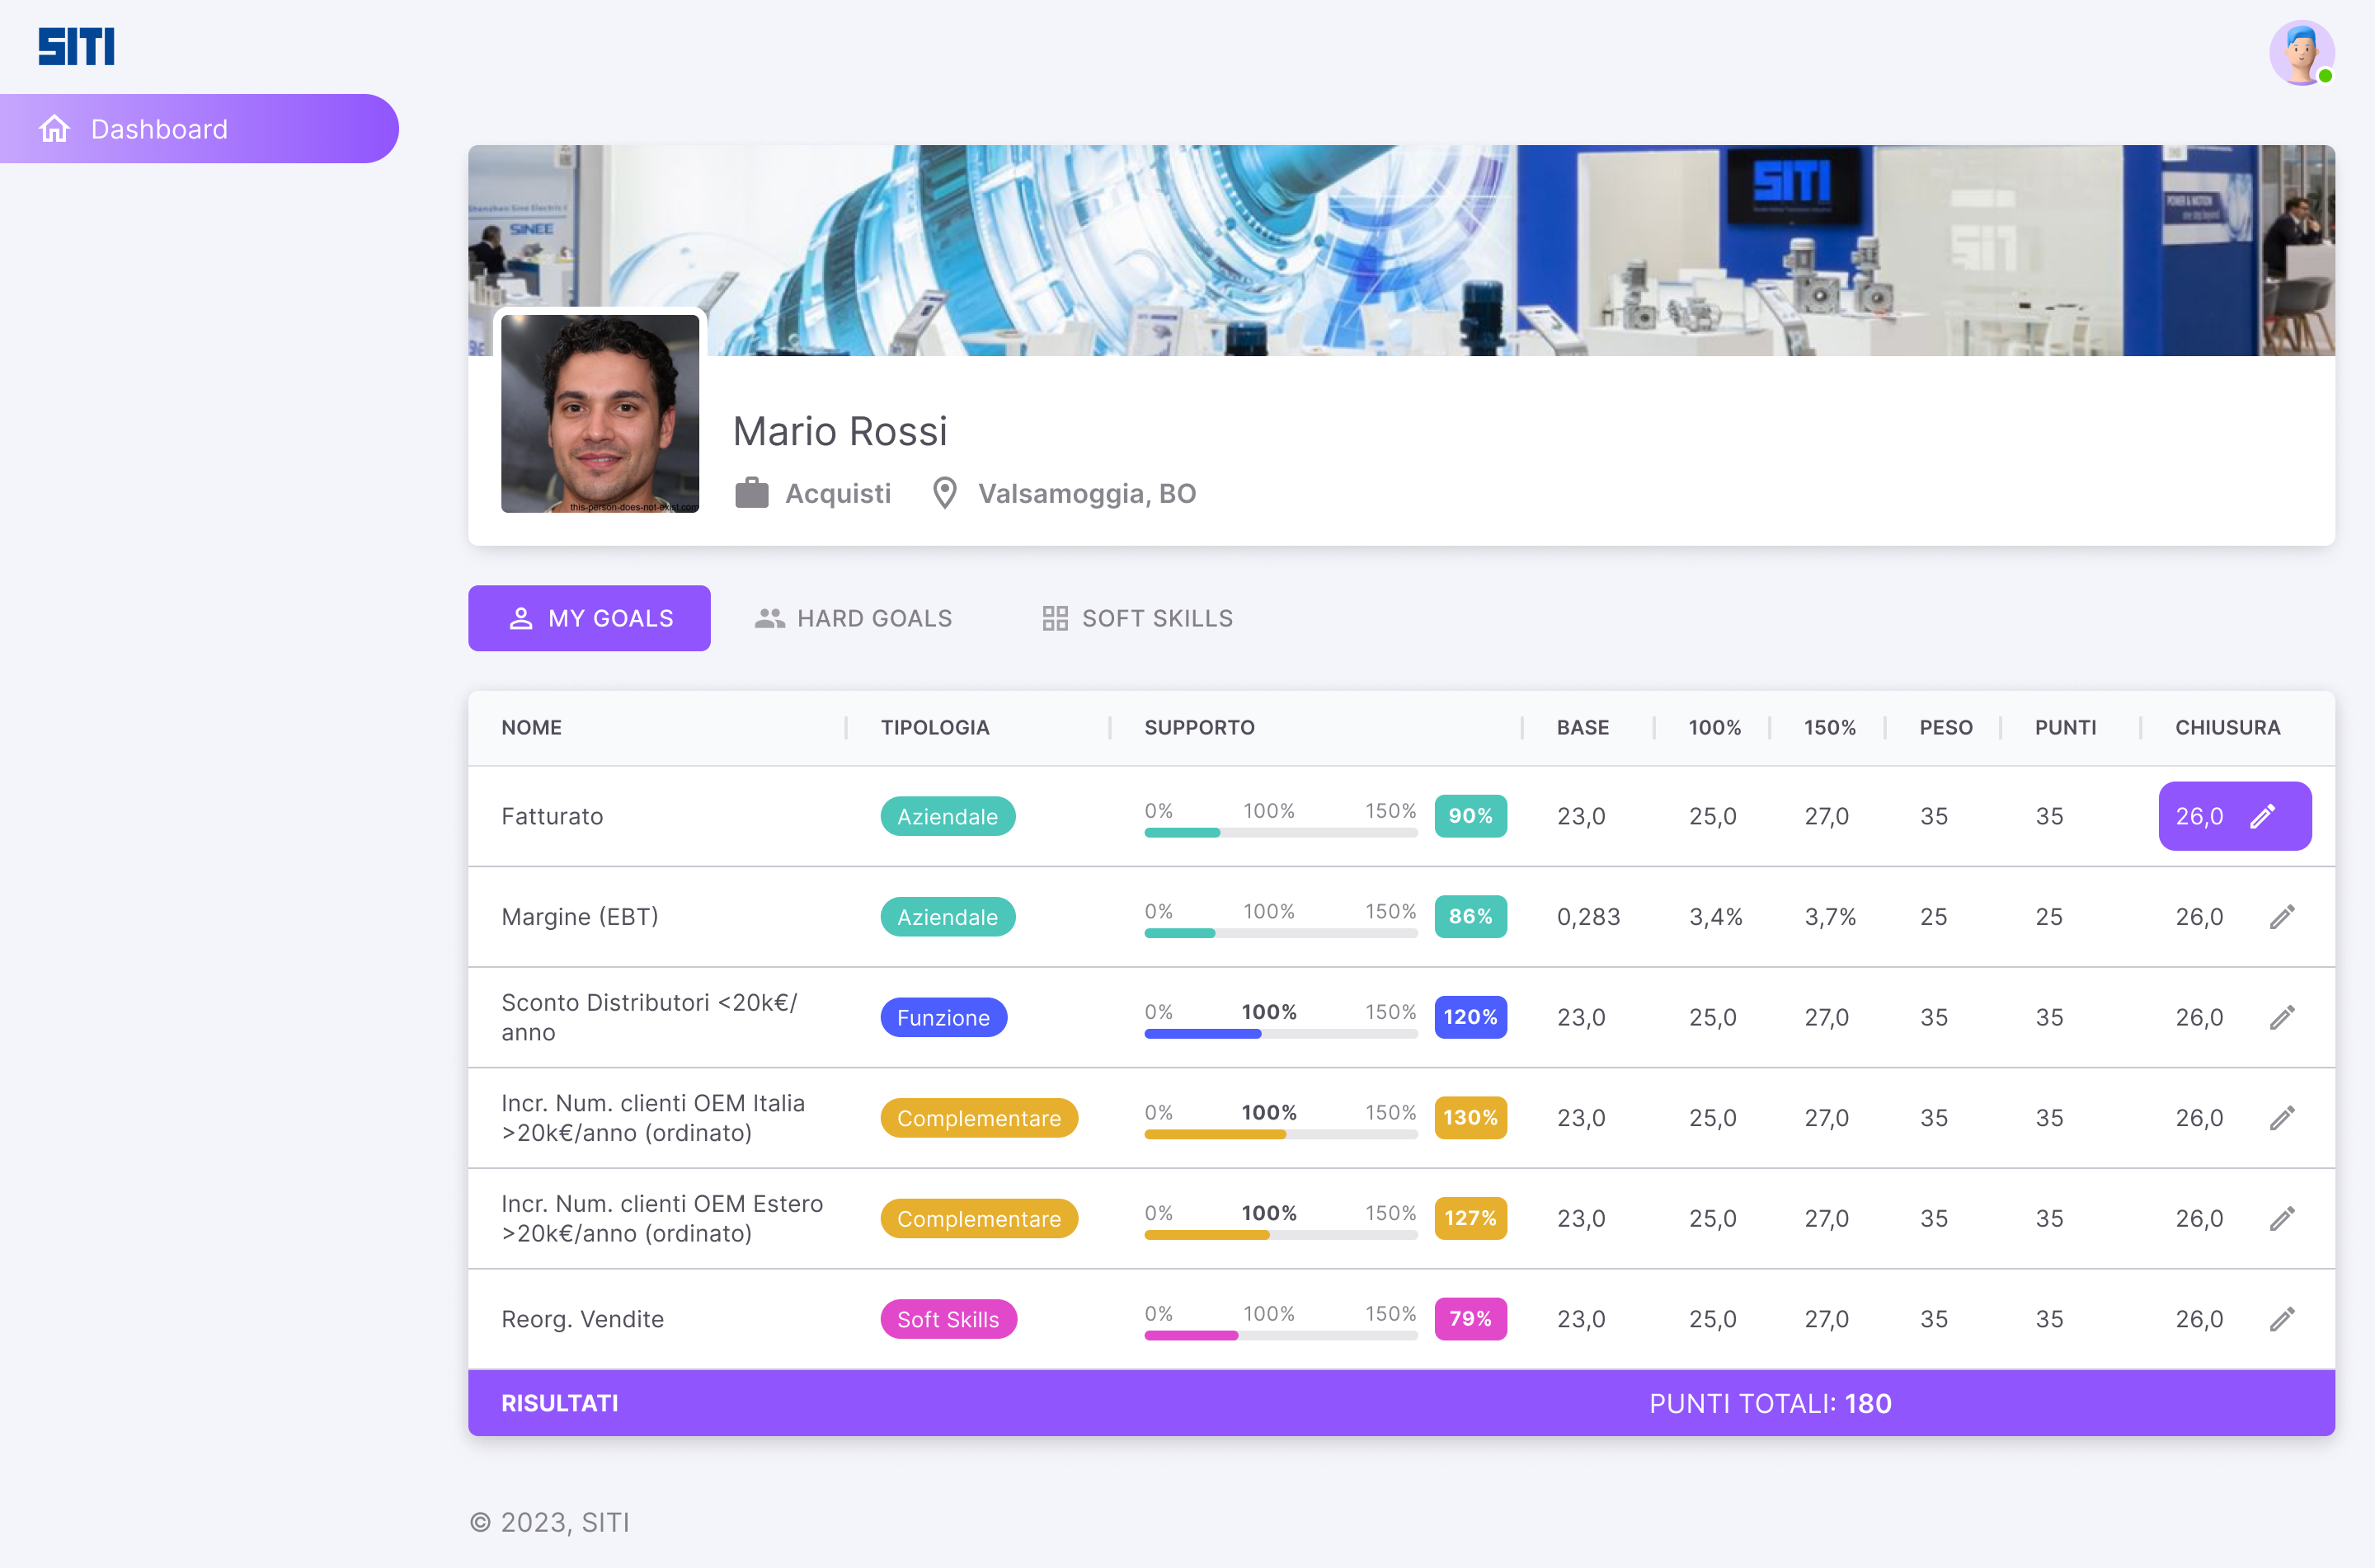
\includegraphics[width=0.8\textwidth]{res/dashboard.png}
    \caption{Dipendente - dashboard dei propri obiettivi}
    \label{fig:dashboard}
\end{figure}

\begin{figure}
    \centering
    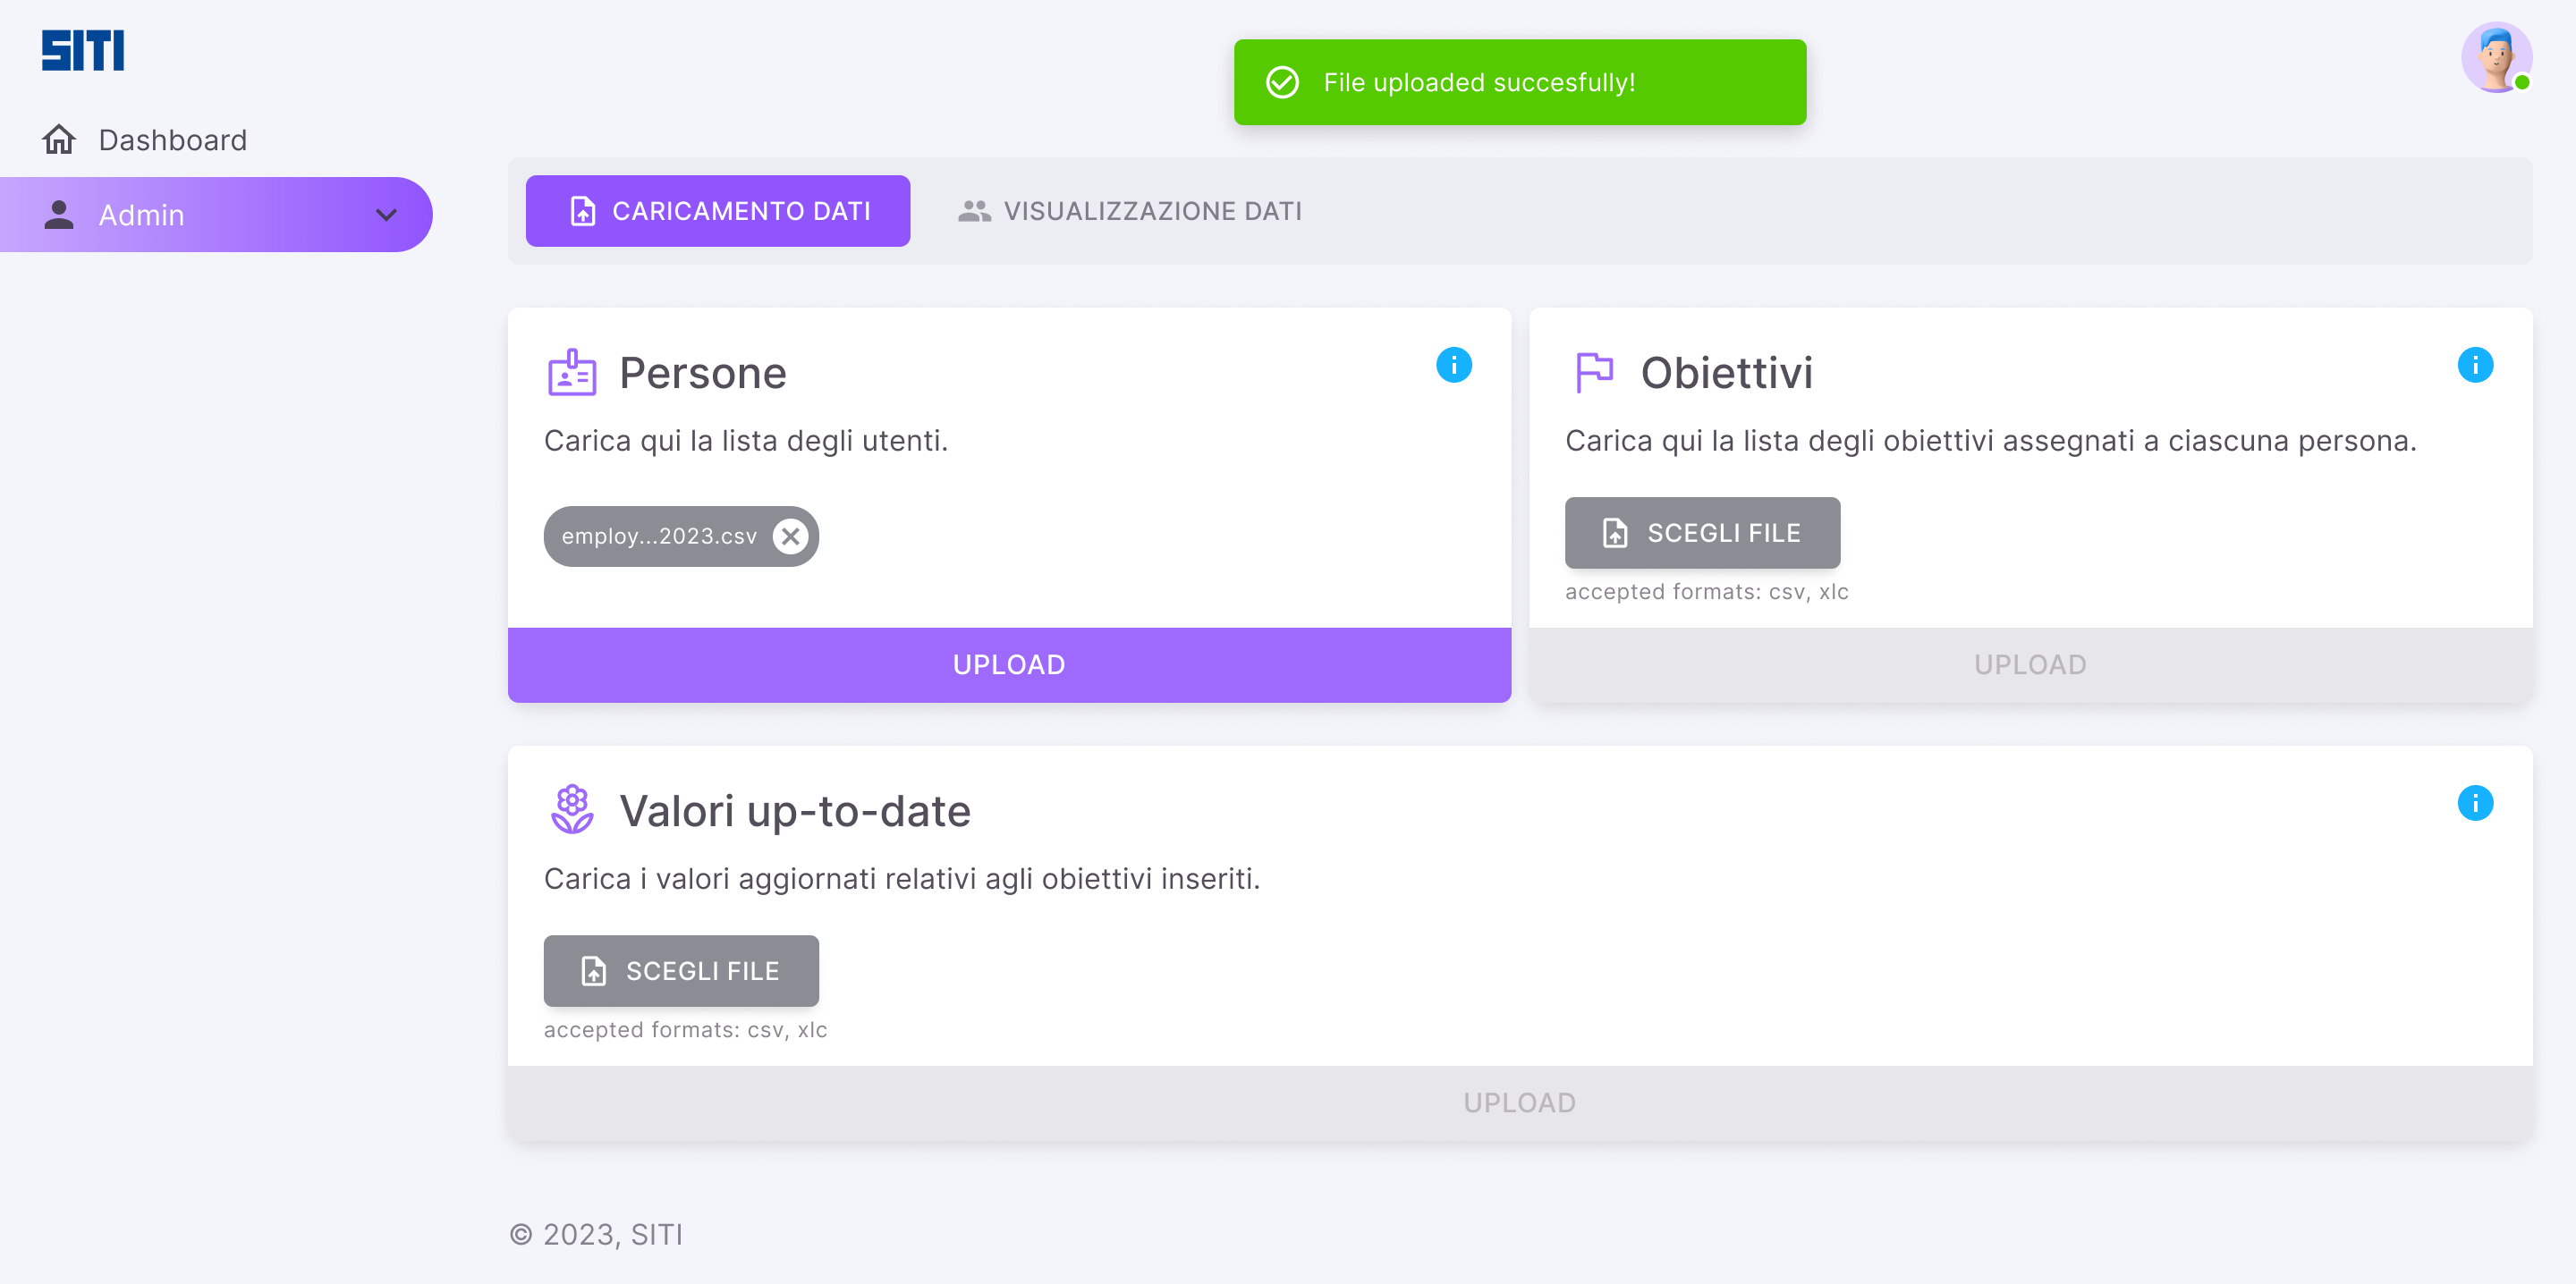
\includegraphics[width=0.8\textwidth]{res/upload.png}
    \caption{Admin - upload dei dati in formato csv}
    \label{fig:upload}
\end{figure}

\begin{figure}
    \centering
    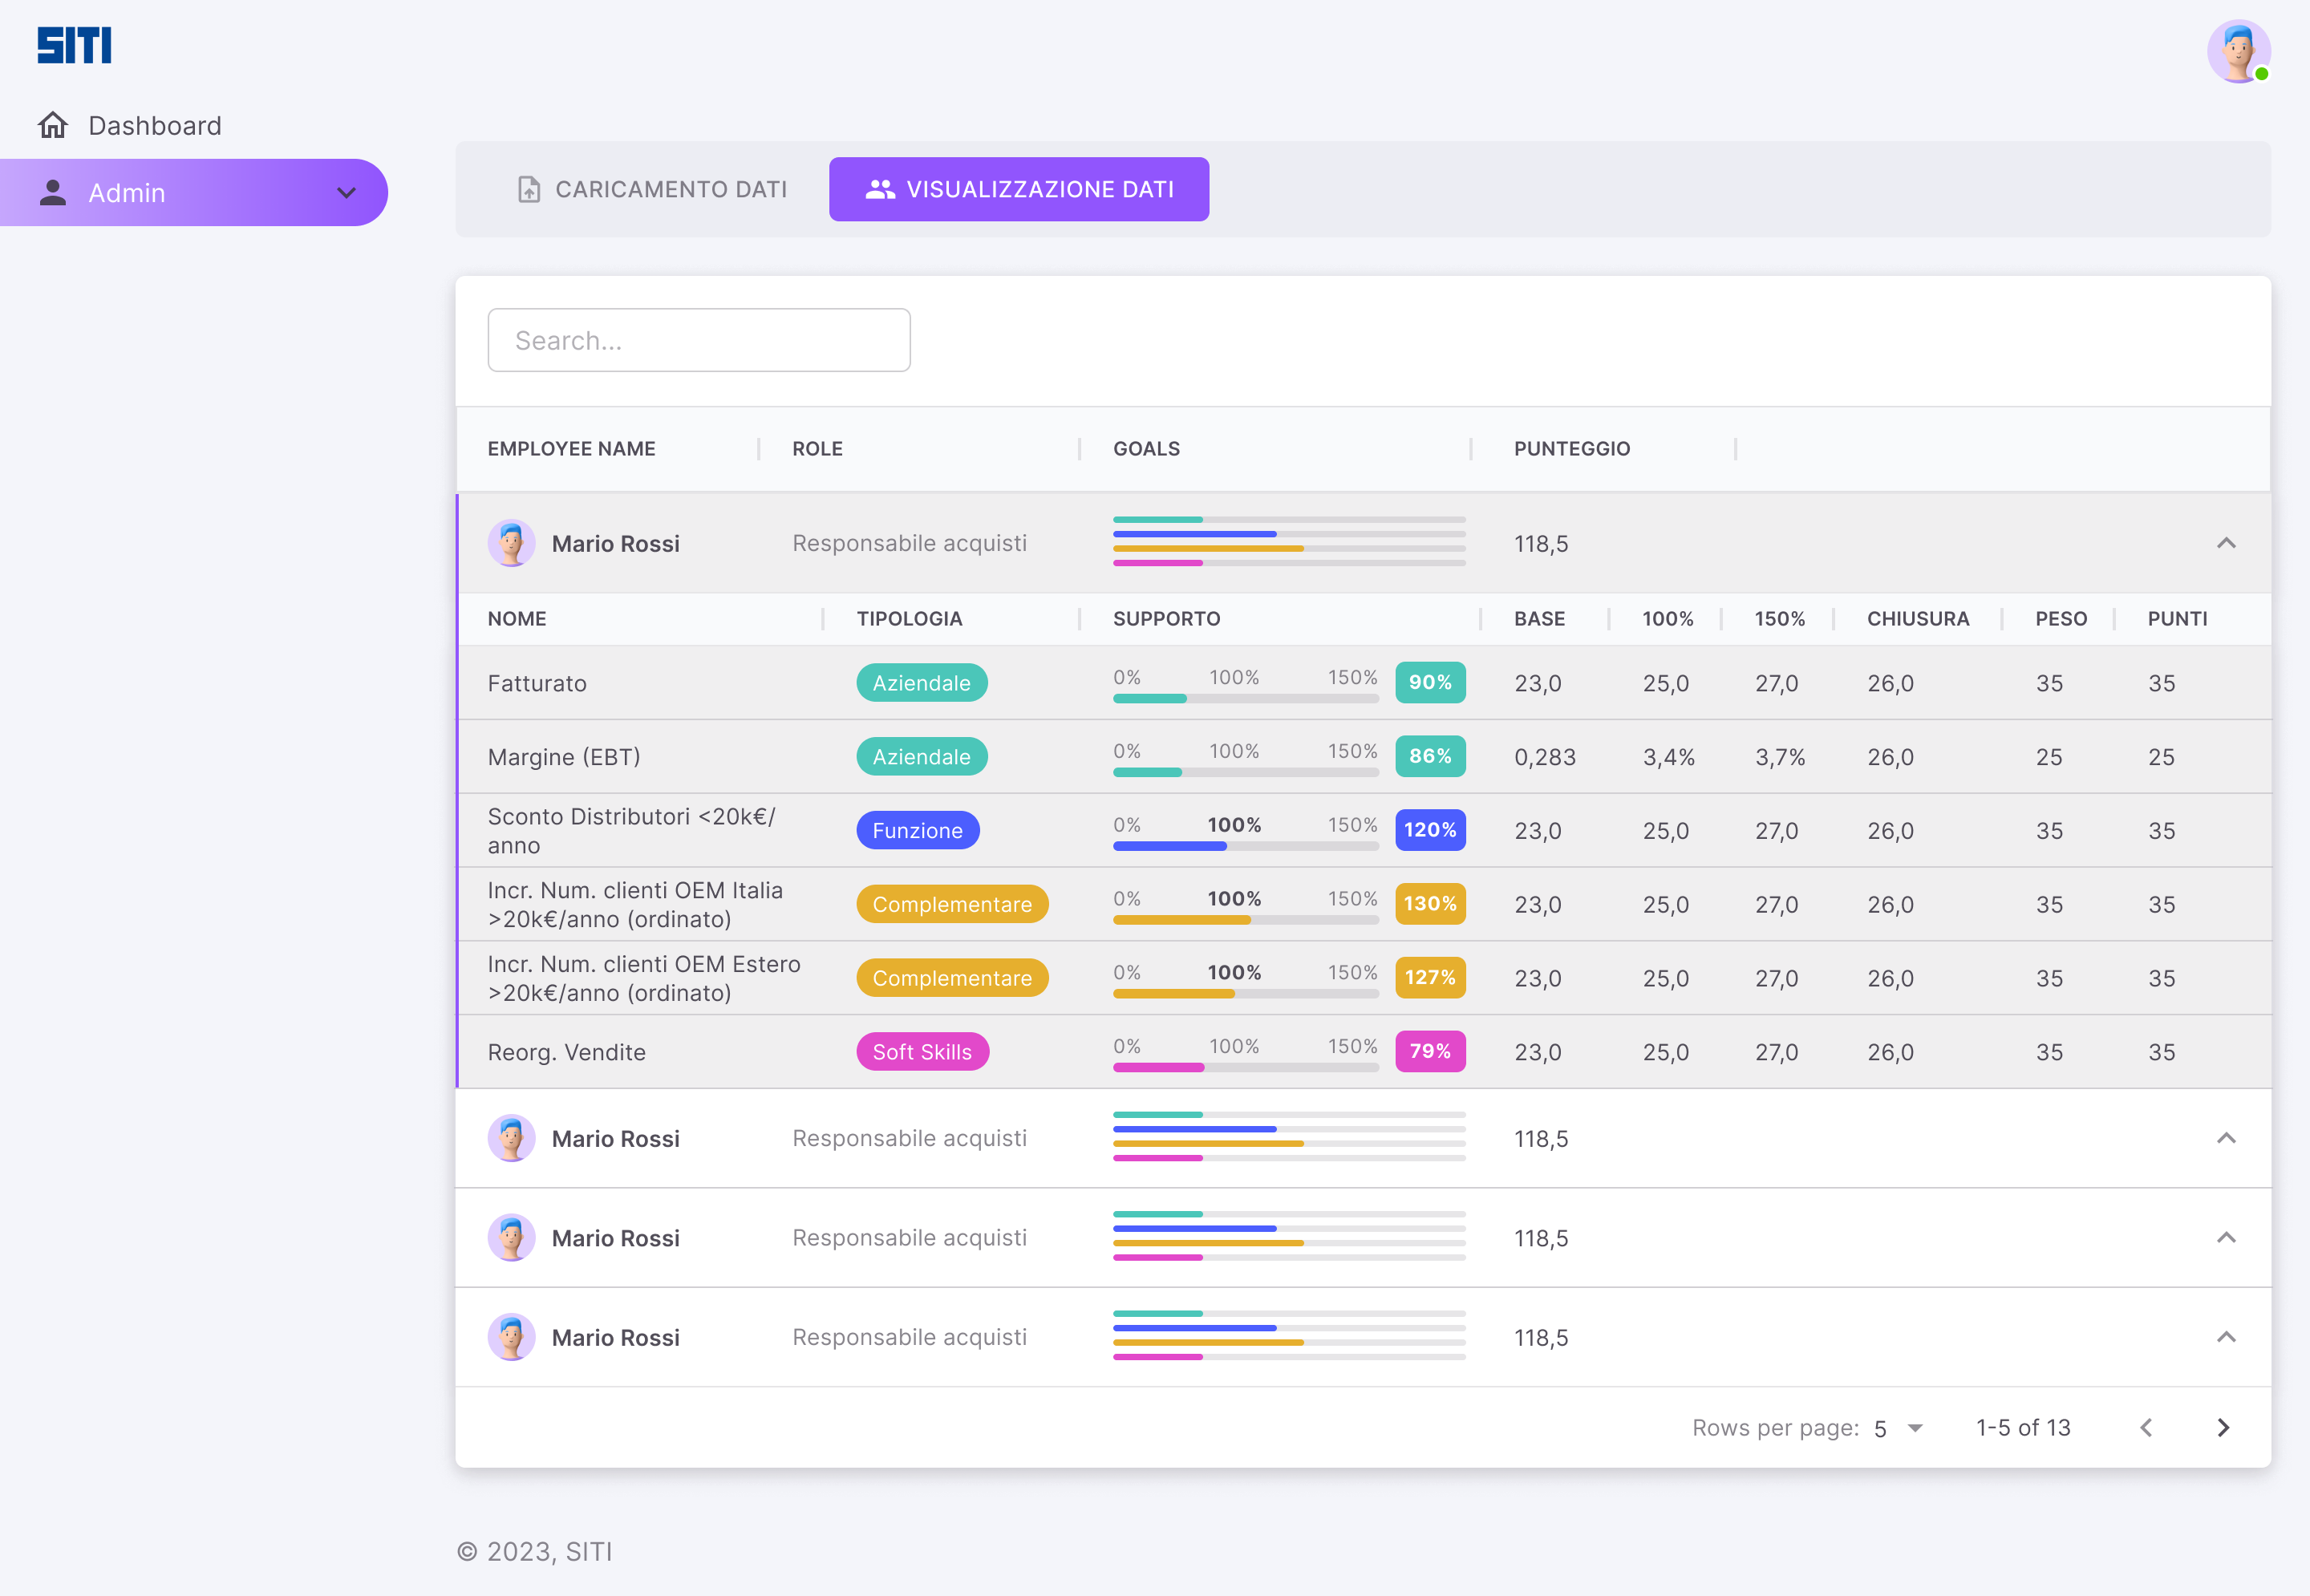
\includegraphics[width=0.8\textwidth]{res/dati.png}
    \caption{Admin - visione d'insieme su tutti i dipendenti}
    \label{fig:dati}
\end{figure}


Il valore di chiusura è il valore raggiunto per l'obiettivo a fine anno. Di default è pari al valore base per l'anno corrente, finchè i dati up-to-date non vengono inseriti.
Nei mockup non era stata prevista la colonna up-to-date. Il design finale dell'app consiste in:
\begin{itemize}
    \item l'admin vede i valori up-to-date di ciascun dipendente
    \item i dipendenti nella propria dashboard, oltre alla colonna up-to-date, hanno a disposizione anche la colonna "chiusura", che è modificabile e consente di simulare valori possibili di chiusura e vedere come cambierebbe il punteggio.
\end{itemize}



\subsection*{Architettura}

\subsubsection{Database schemas}

Il design del database è stato effettuato sulla base delle richieste del cliente.
L'azienda ci ha fornito un file excel contenente tutti i dati che dovevano essere inseriti nel database.

Sulla base di questo file, sono stati creati diversi schemi, ognuno dei quali rappresenta un entità del dominio.

\begin{itemize}
    \item \textbf{User}: contiene i dati degli utenti, ovvero i dipendenti dell'azienda.
    \item \textbf{Credential}: contiene le credenziali degli utenti.
    \item \textbf{Objective}: contiene tutti gli obiettivi che l'azienda si pone.
    \item \textbf{Assigned}: contiene i valori dell'obiettivo, per ogni utente.
    \item \textbf{Default}: contiene i valori di default di ogni obiettivo.
    \item \textbf{Data}: contiene il valore corrente di un utente per un obiettivo.
\end{itemize}

Di seguito vengono mostrati gli schemi del database creati con Mongoose.

\paragraph{Users}

\begin{verbatim}
const userSchema = new Schema({
    username: { type: String, required: true, unique: true},
    name: { type: String, required: true, },
    surname: { type: String, required: true },
    position: { type: String, required: true },
    manager: { type: String },
});
\end{verbatim}

Da notare che l'unico campo non required è il manager. Abbiamo scelto di non renderlo obbligatorio in quanto
ci potrebbero essere delle inconsistenze, o anche solo delle complicazioni, a gestire alcune situazioni.
Inoltre, dopo aver parlato con gli stakeholder, è emerso che la gestione del suddetto campo non è fondamentale 
ai fini del progetto.

La chiave primaria di questo schema è il campo \textit{username}, che è unico.

\paragraph{Credentials}

\begin{verbatim}
const credentialsSchema = new Schema({
    username: { type: String, required: true, unique: true },
    password: { type: String, required: true },
    role: { type: String, required: true }
});
\end{verbatim}

\paragraph{Objectives}

\begin{verbatim}
const objectivesSchema = new Schema({
    name: { type: String, required: true, unique: true },
    type: { type: String, required: true },
})
\end{verbatim}

Questo schema è molto semplice: per ogni obiettivo si salvano nome e tipo. Il nome dell'obiettivo è la 
chiave primaria, ed è unico.

\paragraph{Assigned Objectives}

\begin{verbatim}
const assignedObjectives = new Schema({
    user: { type: String, required: true },
    objective: { type: String, required: true },
    baseValue: { type: Number, required: true },
    value100: { type: Number, required: true },
    value150: { type: Number, required: true },
    weight: { type: Number, required: true },
    year: { type: Number, required: true}
})
\end{verbatim}

Questo schema contiene i valori per ogni obiettivo di ogni utente.
La chiave primaria è composta da \textit{user} e \textit{objective}, in quanto un utente per un determinato 
obiettivo può avere solo un valore. La semantica dei vari campi (value100, value150, etc..) deriva dai dati
forniti dall'azienda.

\paragraph{Default values}

\begin{verbatim}
const defaultsObjectivesSchema = new Schema({
    objective: { type: String, required: true, unique: true },
    defaultBaseValue: { type: Number, required: true },
    default100: { type: Number, required: true },
    default150: { type: Number, required: true },
    defaultWeight: { type: Number, required: true },
})
\end{verbatim}

In questo schema, sono salvati i valori di default per ogni obiettivo. La chiave primaria è il nome dell'obiettivo.
I valori di default sono stati forniti dall'azienda e sono utilizzati in caso non vengano assegnati dei valori 
specifici all'utente.

\paragraph{Data}

\begin{verbatim}
const dataSchema = new Schema({
    objective: { type: String, required: true},
    username: { type: String, required: true },
    date: { type: Date, required: true},
    value: { type: Number, required: true },
})
\end{verbatim}

Nel Data schema sono contenuti i valori reali di un utente per un obiettivo in una determinata data.

\subsubsection{API}

Le API utilizzano Next.js API routes. Questo framework permette di creare delle API RESTful in modo molto semplice.

Di sono mostrate le routes create:

\begin{table}[]
    \begin{tabular}{ll}
    users/put             & Aggiunge uno o più utenti al database (gli utenti già esistenti vengono aggiornati).                     \\
    users/get             & Recupera un utente dal database (nel caso non venga specificato uno username, ritorna tutti gli utenti). \\
    users/delete          & Rimuove un utente dal database e come manager di altri utenti, insieme agli obiettivi a lui assegnati.   \\
    users/update/manager  & Aggiorna il manager di un utente.                                                                        \\
    users/update/position & Aggiorna la posizione di un utente.                                                                      \\
    objectives/put        & Aggiunge uno o più obiettivi al database (gli obiettivi già esistenti vengono aggiornati)                \\
    objectives/get        & Recupera un obiettivo dal database (nel caso non venga specificato un nome obiettivo, li ritorna tutti)  \\
    objectives/delete     & Rimuove un obiettivo dal database.                                                                       \\
    assigned/put          & Assegna un obiettivo ad un utente, o più obiettivi a più utenti.                                         \\
    assigned/get          & Dato un utente, recupera tutti gli obiettivi a lui assegnati.                                            \\
    assigned/deleteAll    & Rimuove tutti gli obiettivi assegnati.                                                                   \\
    data/put              & Aggiunge (o aggiorna) i valori per un utente, relativi ad un obiettivo.                                  \\
    data/get              & Recupera i valori di un utente per un obiettivo.                                                         \\
    data/deleteAll        & Rimuove tutti i valori                                                                                   \\
    auth/me               & TODO                                                                                                     \\
    auth/login            & TODO                                                                                                    
    \end{tabular}
\end{table}